\part{RNNs and Transformers}
\chapter{Introduction to RNNs}
In this lesson, we will learn about \textbf{Recurrent Neural Networks (RNNs)}. \newline

The neural network architectures you've seen so far were trained using the current inputs only. We did not consider previous inputs when generating the current output. In other words, our systems did not have any \textbf{memory} elements. RNNs address this basic and essential issue by using \textbf{memory} (i.e., past inputs to the network) when producing the current output. \newline

\href{https://www.youtube.com/watch?v=AIQEqg6F38A&t=1s&ab_channel=Udacity}{Youtube}

Temporal dependencies = current output depends on current input and past inputs 

\includegraphics[width=0.75\linewidth]{img//rnn/nn_rnn.png}

\section{A bit of history}

How did the theory behind RNN evolve? Where were we a few years ago and where are we now? \newline

\href{https://www.youtube.com/watch?v=HbxAnYUfRnc&ab_channel=Udacity}{Youtube} \newline

As mentioned in this video, RNNs have a key flaw, as capturing relationships that span more than 8 or 10 steps back is practically impossible. This flaw stems from the "\textbf{vanishing gradient}" problem in which the contribution of information decays geometrically over time. \newline

What does this mean? \newline

As you may recall, while training our network, we use \textbf{backpropagation}. In the backpropagation process, we adjust our weight matrices using a \textbf{gradient}. In the process, gradients are calculated by continuous multiplications of derivatives. The value of these derivatives may be so small that these continuous multiplications may cause the gradient to practically "vanish." \newline

\textbf{LSTM} is one option to overcome the Vanishing Gradient problem in RNNs. \newline

As mentioned in the video, Long Short-Term Memory Cells (LSTMs) and Gated Recurrent Units (GRUs) give a solution to the vanishing gradient problem by helping us apply networks that have temporal dependencies. \newline

More information about GRUs can be found \href{https://towardsdatascience.com/understanding-gru-networks-2ef37df6c9be}{\textbf{here}}. Focus on the overview titled: \textbf{GRUs}. \newline

\subsubsection{Extra Resources}

\begin{itemize}
    \item \href{https://en.wikipedia.org/wiki/Vanishing_gradient_problem}{\textbf{Vanishing Gradient Problem}}
    \item \href{https://socratic.org/algebra/exponents-and-exponential-functions/geometric-sequences-and-exponential-functions}{\textbf{Geometric Series}}
    \item \href{https://en.wikipedia.org/wiki/Time_delay_neural_network}{\textbf{TDNN (Time delay neural network)}}
    \item Here is the original \href{http://onlinelibrary.wiley.com/doi/10.1207/s15516709cog1402_1/abstract}{\textbf{Elman Network}} publication from 1990. This link is provided here as it's a significant milestone in the world of RNNs. To simplify things a bit, you can take a look at the following \href{https://en.wikipedia.org/wiki/Recurrent_neural_network\#Elman_networks_and_Jordan_networks}{\textbf{additional info}}.
    \item In this \href{http://www.bioinf.jku.at/publications/older/2604.pdf}{\textbf{LSTM}} link, you will find the original paper written by \href{https://en.wikipedia.org/wiki/Sepp_Hochreiter}{\textbf{Sepp Hochreiter}} and \href{http://people.idsia.ch/~juergen/}{\textbf{Jürgen Schmidhuber}}. Don't get into all the details just yet. We will cover all of this later!
\end{itemize}


\section{RNN Applications}

The world's leading tech companies use RNNs, particularly LSTMs, in their applications. Let's take a look at a few. \newline

\href{https://www.youtube.com/watch?v=6JbTNARuKII&ab_channel=Udacity}{Youtube}

There are so many interesting applications; let's look at a few more!

\begin{itemize}
    \item Are you into gaming and bots? Check out the \href{https://openai.com/research/dota-2}{\textbf{DotA 2 bot by Open AI}}
    \item How about \href{https://www.youtube.com/watch?time_continue=1&v=0FW99AQmMc8}{\textbf{automatically adding sounds to silent movies?}}
    \item Amazon's voice-to-text using high-quality speech recognition, \href{https://aws.amazon.com/lex/faqs/}{\textbf{Amazon Lex}}.
    \item Facebook uses RNN and LSTM technologies for \href{https://code.facebook.com/posts/1827693967466780/building-an-efficient-neural-language-model-over-a-billion-words/}{\textbf{building language models}}
    \item Netflix also uses RNN models - \href{https://arxiv.org/pdf/1511.06939.pdf}{\textbf{here is an interesting read}}
\end{itemize}

\section{Recurrent Neural Networks}
\href{https://www.youtube.com/watch?v=ofbnDxGSUcg&ab_channel=Udacity}{Youtube} \newline

RNNs are based on the same principles as those behind FFNNs, which is why we spent so much time reminding ourselves of the feedforward and backpropagation steps used in the training phase.

    \includegraphics[width=0.5\linewidth]{img//rnn//intro/image1.png}

Current output \(\overline{y}\) depends not only on the current input \(\overline{x}\) but also on the memory element \(\overline{s}\) which takes into account past inputs. Example: Predicting the next word in the sentence. Which requires at the last few words rather than only the current one.

There are two main differences between FFNNs and RNNs. The Recurrent Neural Network uses:

\begin{itemize}
    \item \textbf{sequences} as inputs in the training phase, and
    \item \textbf{memory} elements
\end{itemize}
Memory is defined as the output of hidden layer neurons, which will serve as additional input to the network during the next training step.

    \includegraphics[width=1\linewidth]{img//rnn//intro/image2.png}

The first difference , is the manner by which we define our inputs and outputs. Instead of training the network using a single-input, single-output at each time step, we train with sequences since previous inputs matter. The second difference, stems from the memory elements that RNN's host. Current inputs, as well as activations of neurons serve as inputs to the next time step.

\includegraphics[width=1\linewidth]{img//rnn//intro/image3.png}

In feedforward neural networks,we saw a flow of information from the input to the output without any feedback.

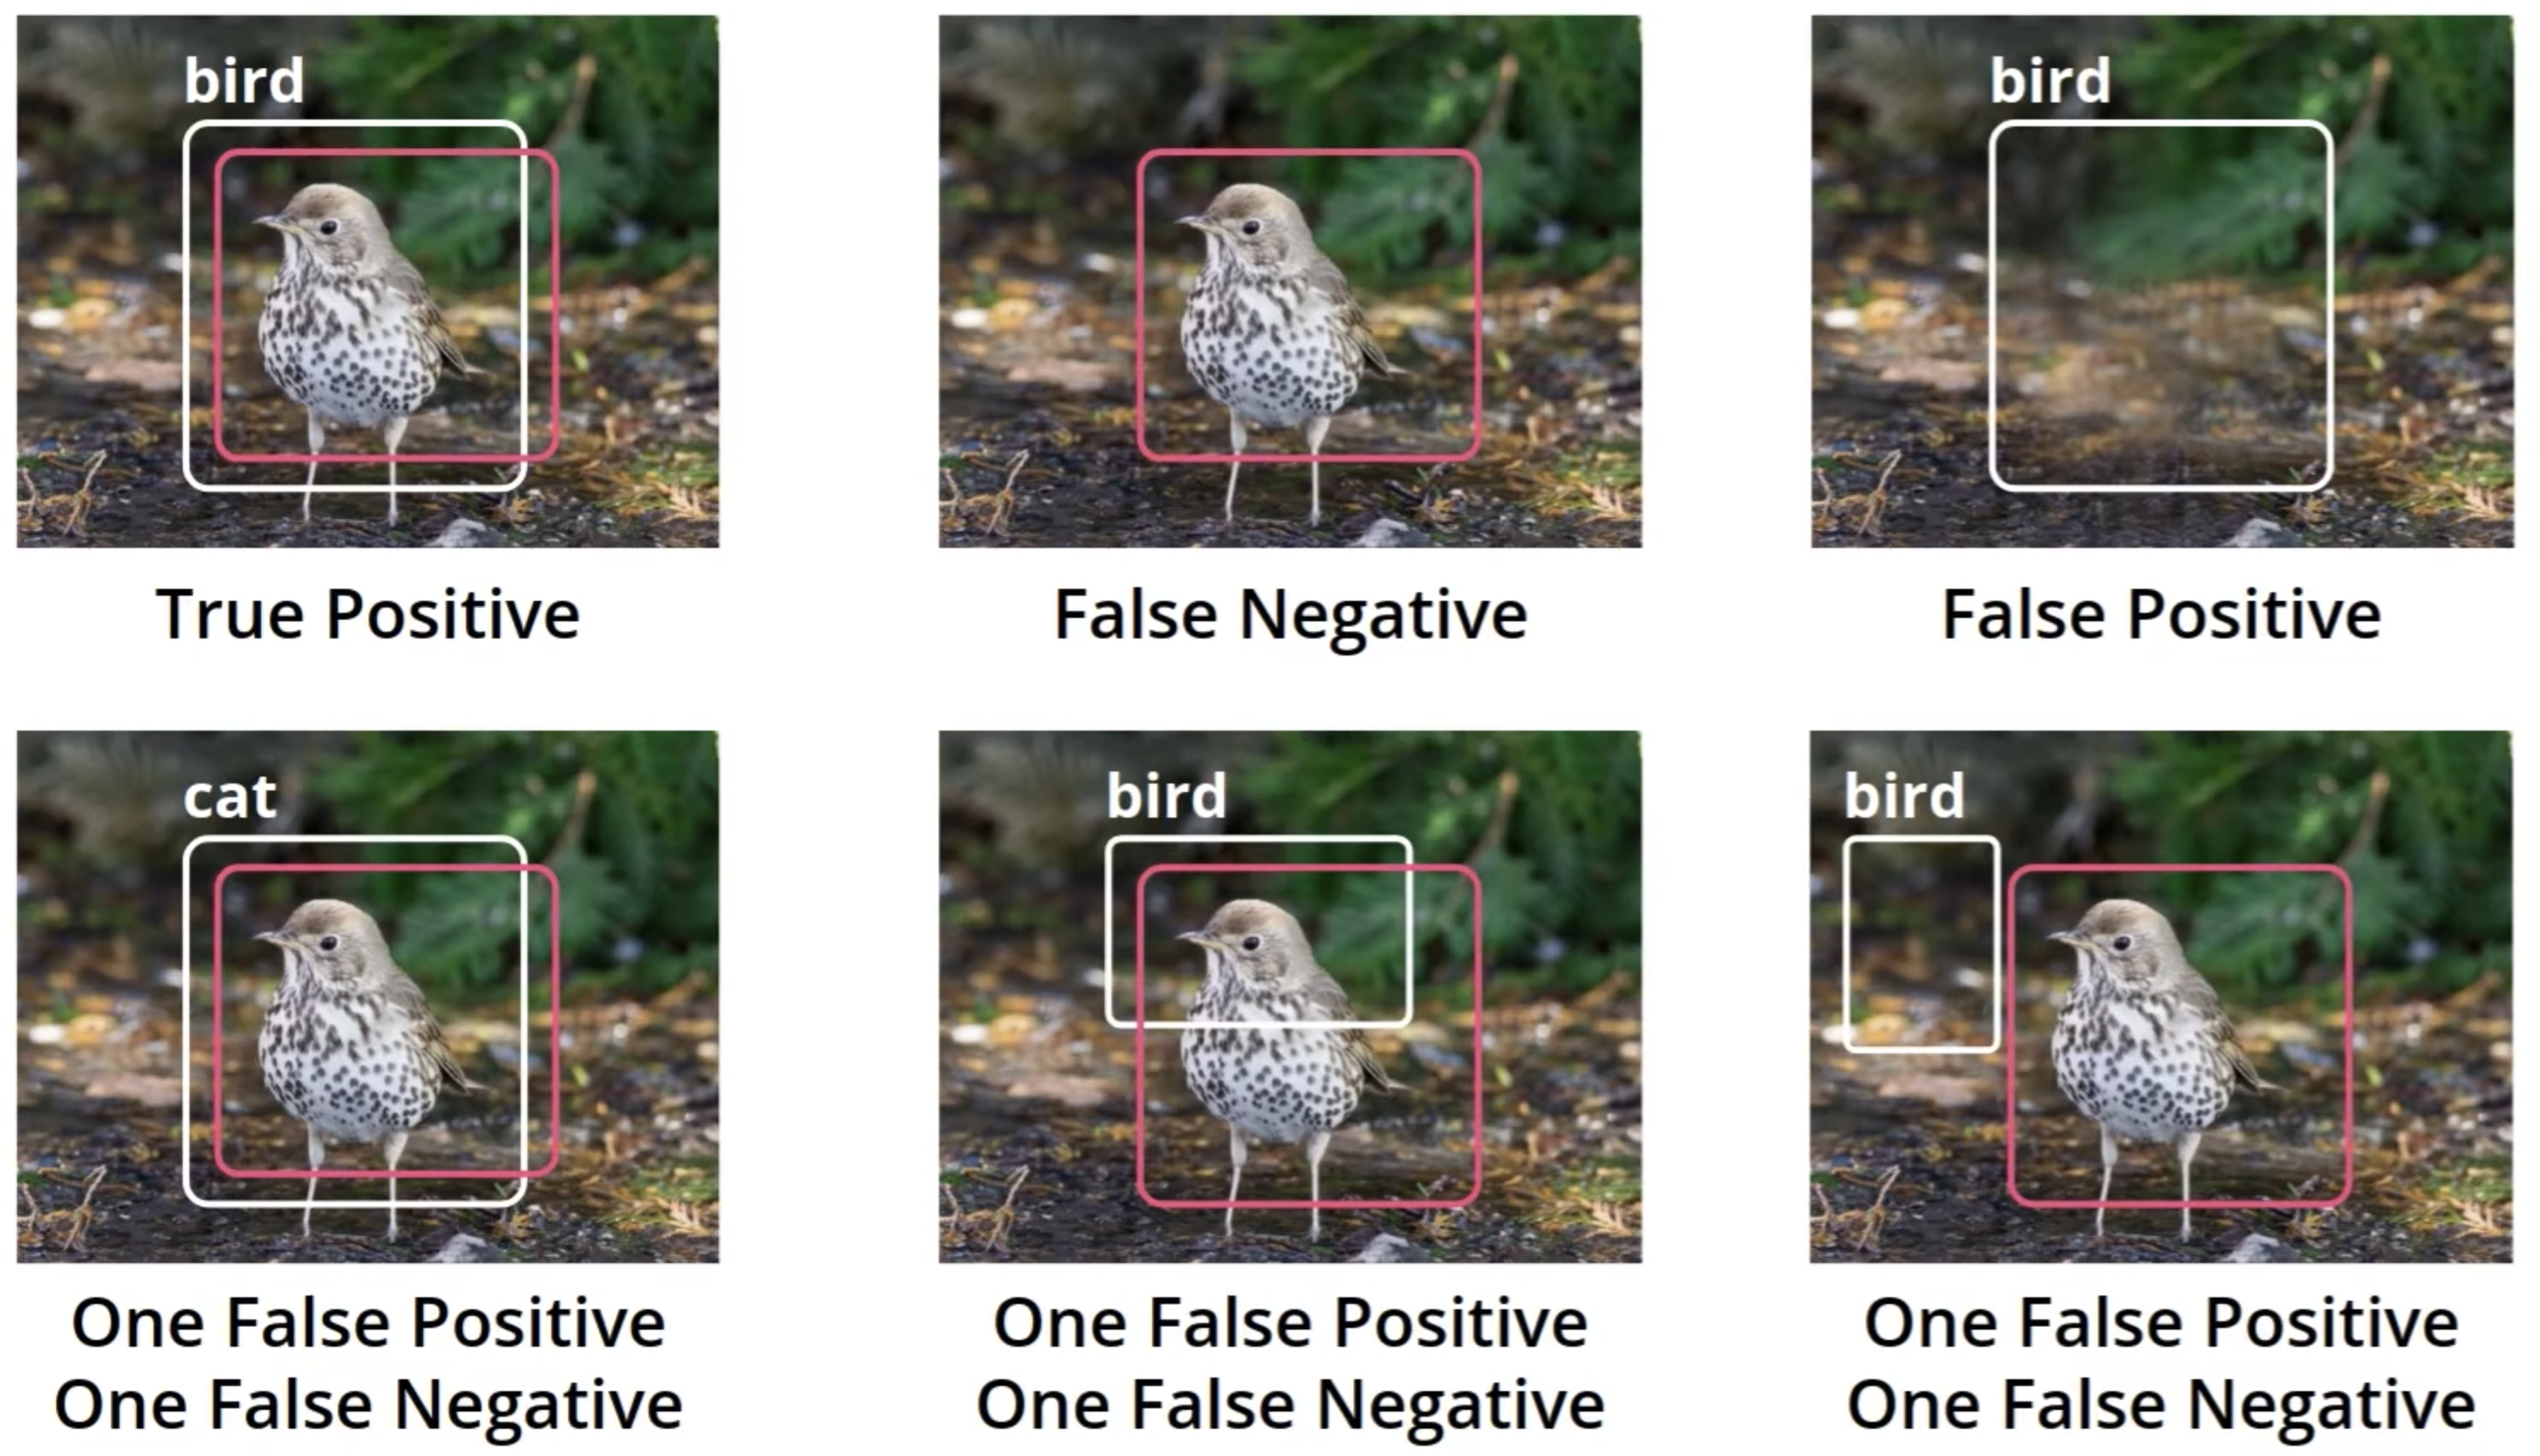
\includegraphics[width=0.75\linewidth]{img//rnn//intro/image.png}

Now, that feedforward scheme changes, and includes the feedback or memory elements. We will consider memory defined, as the output of the hidden layer, which will serve as an additional input to the network at the following training step. We will no longer use H as the output of the hidden layer, but S for state, referring to a system with memory. The basic scheme of RNN is called Simple RNN, and is also known as an Elman Network. \newline

The basic three layer neural network with feedback that serve as memory inputs is called the \textbf{Elman Network} and is depicted in the following picture:

\includegraphics[width=0.5\linewidth]{img//rnn//intro/screen-shot-2017-11-06-at-1.40.14-pm.png}
\captionof{figure}{Elman Network, source: Wikipedia}

\subsection{RNN - Folded and Unfolded Model}
\href{https://www.youtube.com/watch?v=wsif3p5t7CI&ab_channel=Udacity}{Youtube} \newline

In FFNN the output at any time \textit{t}, is a function of the current input and the weights. This can be easily expressed using the following equation: 
\begin{equation}
    \overline{y}_t = F(\overline{x}_t, W)
\end{equation}

We assume that the inputs are independent of each other. Therefore, there is no significance to the sequence. So we train the system by randomly drawing inputs and target pairs. \newline

In RNNs, our output at time t, depends not only on the current input and the weight, but also on previous inputs. In this case the output at time t will be defined as:

\begin{equation}
    \overline{y}_t = F(\overline{x}_t, \overline{x}_{t-1}, \overline{x}_{t-2}, \overline{x}_{t-t_0}, W)
\end{equation}

This is the RNN \textbf{folded model}:

\includegraphics[width=0.5\linewidth]{img//rnn//intro/screen-shot-2017-11-06-at-2.09.07-pm.png}
\captionof{figure}{The RNN folded model}

In this picture, \(\overline{x}\) represents the input vector, \(\overline{y}\) represents the output vector and \(\overline{s}\) denotes the state vector. \newline

 \(W_x\) is the weight matrix connecting the inputs to the state layer. \newline

\(W_y\) is the weight matrix connecting the state layer to the output layer. \newline

\(W_s\) represents the weight matrix connecting the state from the previous timestep to the state in the current timestep. \newline

The model can also be "unfolded in time". The \textbf{unfolded model} is usually what we use when working with RNNs. \newline

\href{https://www.youtube.com/watch?v=xLIA_PTWXog&ab_channel=Udacity}{Youtube} \newline

\includegraphics[width=01\linewidth]{img//rnn//intro/screen-shot-2017-11-06-at-2.38.51-pm.png}
\captionof{figure}{The RNN unfolded model}


\subsubsection{The Unfolded Model}

The Unfolded Model is useful for visualizing the RNN. This is because The Unfolded Model provides a more straightforward way to separate and understand the parts of the RNN. \newline

Here's how the unfolded model helps us understand RNNs:

\begin{itemize}
    \item Separates the State Vector from the Input Vector to simplify the diagram
    \item Shows how both the State Vector and the Input Vector interact with the same weights
    \item Makes it easier to understand how the State at T-1 and the Input Vector at T produce the Output at T
\end{itemize}
In RNNs the state layer depended on the current inputs, their corresponding weights, the activation function and \textbf{also} on the previous state:

\begin{equation}
    \overline{s}_t = \Phi(\overline{x}_t W_x + \overline{s}_{t-1} W_s)
\end{equation}

The output vector is calculated exactly the same as in FFNNs. It can be a linear combination of the inputs to each output node with the corresponding weight matrix \(W_y\), or a softmax function of the same linear combination.

\begin{equation}
    \begin{split}
        \overline{y}_t = \overline{s}_t W_y \\
        \textnormal{or} \\
        \overline{y}_t = \sigma(\overline{s}_t W_y)
    \end{split}  
\end{equation}

\section{RNN Example}

In this example, we will illustrate how RNNs can help detect sequences. When detecting a sequence, the system must remember the previous inputs, so it makes sense to use a recurrent network. \newline

If you are unfamiliar with sequence detection, the idea is to see if a specific pattern of inputs has entered the system. In our example, the pattern will be the word U,D,A,C,I,T,Y. \newline

\href{https://www.youtube.com/watch?v=MDLk3fhpTx0&ab_channel=Udacity}{Youtube} 


\section{Backpropagation Through Time - I}

We are now ready to understand how to train the RNN.

When we train RNNs we also use backpropagation, but with a conceptual change. The process is similar to that in the FFNN, with the exception that we need to consider previous time steps, as the system has memory. This process is called \textbf{Backpropagation Through Time (BPTT)}.

We will use the \href{https://en.wikipedia.org/wiki/Mean_squared_error}{\textbf{MSE loss function}} to explain the BPTT. Recall that Mean Squared error \(E_t = (\overline{d}_t - \overline{y}_t)^2\)

where
\begin{itemize}
     \item \(E_t\)represents the output error at time t
     \item \(d_t\) represents the desired output at time t
     \item \(y_t\) represents the calculated output at time t
\end{itemize}
\href{https://www.youtube.com/watch?v=eE2L3-2wKac&ab_channel=Udacity}{Youtube} \newline

In \textbf{BPTT} we train the network at timestep t and take into account all of the previous timesteps. Let's understand this with the help of an example. \newline

In this example, we will focus on the \textbf{BPTT} process for time step t=3. You will see that to adjust all three weight matrices, \(W_x, W_s,\) and \(W_y\), we need to consider timestep 3 as well as timestep 2 and timestep 1. \newline

As we are focusing on timestep t=3, the Loss function will be:  \(E_3 = (\overline{d}_3 - \overline{y}_3)^2\)

\includegraphics[width=0.5\linewidth]{img//rnn//intro/screen-shot-2017-11-27-at-1.43.36-pm.png}
\captionof{figure}{The Folded Model at Timestep 3}

To update each weight matrix, we need to find the partial derivatives of the Loss Function at time 3, as a function of all of the weight matrices. We will modify each matrix using gradient descent while considering the previous timesteps.

\includegraphics[width=0.5\linewidth]{img//rnn//intro/screen-shot-2017-11-27-at-1.46.43-pm.png}
\captionof{figure}{Gradient Considerations in the Folded Model}

We will now unfold the model. You will see that unfolding the model in time is very helpful in visualizing the number of steps (translated into multiplication) needed in the Backpropagation Through Time process. These multiplications stem from the chain rule and are easily visualized using this model.


\section{Backpropagation Through Time - II}

\subsubsection{Unfolding the model in time}

In the following video we will understand how to use Backpropagation Through Time (BPTT) when adjusting two weight matrices:

\begin{itemize}
    \item \(W_y\)- the weight matrix connecting the state of the output
    \item \(W_s\) - the weight matrix connecting one state to the next state
\end{itemize}
\href{https://www.youtube.com/watch?v=bUU9BEQw0IA&ab_channel=Udacity}{Youtube} \newline



\textbf{Gradient calculations needed to adjust \(W_y\)} \newline

The partial derivative of the Loss Function concerning \(W_y\) is found by a simple one-step chain rule: (Note that in this case, we do not need to use BPTT. Visualization of the calculations path can be found in the video).

\[\frac{\partial E_3}{\partial W_y} = \frac{\partial E_3}{\partial \overline{y}_3} \frac{\partial \overline{y}_3}{\partial W_y}\]
\captionof{figure}{Chain rule for calculating partial derivative of loss}

\[\frac{\partial E_N}{\partial W_y} = \frac{\partial E_N}{\partial \overline{y}_N} \frac{\partial \overline{y}_N}{\partial W_y}\]
\captionof{figure}{Chain rule for calculating partial derivative of loss (N steps)}

\textbf{Gradient calculations needed to adjust \(W_s\)} \newline

We still need to adjust \(W_s\) the weight matrix connecting one state to the next and \(W_x\) the weight matrix connecting the input to the state. We will arbitrarily start with \(W_s\). \newline

To understand the \textbf{BPTT} process, we can simplify the unfolded model. We will focus on the contributions of \(W_s\) to the output, the following way:

\includegraphics[width=0.5\linewidth]{img//rnn//intro/screen-shot-2017-11-27-at-2.00.15-pm.png}
\captionof{figure}{Simplified Unfolded model for Adjusting Ws}

When calculating the partial derivative of the Loss Function for \(W_s\), we need to consider all of the states contributing to the output. In the case of this example, it will be states \(\overline{s}_3\) which depends on its predecessor \(\overline{s}_2\) which depends on its predecessor \(\overline{s}_1\), the first state. \newline

In \textbf{BPTT}, we will consider every gradient stemming from each state, \textbf{accumulating} all of these contributions. \newline

At timestep t=3, the contribution to the gradient stemming from \(\overline{s}_3\), \(\overline{s}_2\), and \(\overline{s}_1\) is the following: \newline

\textbf{Note: Notice the use of the chain rule here. If you need, go back to the video to visualize the calculation path.}

\includegraphics[width=0.5\linewidth]{img//rnn//intro/bptt_eq.jpeg}
\captionof{figure}{Final gradient calculation in the BPTT algorithm (considering 3 timesteps)}

Generalizing for N timesteps, we get: \[\frac{\partial E_N}{\partial W_s} = \sum_{i=1}^N \frac{\partial E_N}{\partial \overline{y}_N} \frac{\partial \overline{y}_N}{\partial \overline{s}_i} \frac{\partial \overline{s}_i}{\partial W_s}\] \captionof{figure}{Final gradient calculation in the BPTT algorithm (considering N timesteps)}

We still need to adjust \textbf{\(W_x\)}, the weight matrix connecting the nuput to the state.

\subsubsection{Adjusting / Updating \(W_x\)}
\href{https://www.youtube.com/watch?v=uBy_eIJDD1M&ab_channel=Udacity}{Youtube} \newline

When calculating the partial derivative of the Loss Function concerning to \(W_x\) we need to consider, again, all of the states contributing to the output. As we saw before, in the case of this example, it will be states \(\overline{s}_3\), which depend on its predecessor \(\overline{s}_2\), which depends on its predecessor \(\overline{s}_1\), the first state.

\includegraphics[width=0.5\linewidth]{img//rnn//intro/screen-shot-2017-11-08-at-3.43.34-pm.png}
\captionof{figure}{Simplified Unfolded model for Adjusting Wx}

After considering the contributions from all three states: \(\overline{s}_3\), \(\overline{s}_2\) and \(\overline{s}_1\), we will \textbf{accumulate} them to find the final gradient calculation. \newline

The following equation is the gradient contributing to the adjustment of \textbf{\(W_x\) }using \textbf{Backpropagation Through Time}:

\begin{equation}
    \begin{split}
        \frac{\partial E_3}{\partial W_x} & = \frac{E_3}{\partial \overline{y}_3} \frac{\partial \overline{y}_3}{\partial \overline{s}_3} \frac{\partial \overline{s}_3}{\partial W_x} + \\
        & = \frac{E_3}{\partial \overline{y}_3} \frac{\partial \overline{y}_3}{\partial \overline{s}_3} \frac{\partial \overline{s}_3}{\partial \overline{s}_2} \frac{\partial \overline{s}_2}{\partial W_x} + \\
        & = \frac{E_3}{\partial \overline{y}_3} \frac{\partial \overline{y}_3}{\partial \overline{s}_3} \frac{\partial \overline{s}_3}{\partial \overline{s}_2} \frac{\partial \overline{s}_2}{\partial \overline{s}_1} \frac{\partial \overline{s}_1}{\partial W_x}
    \end{split}
\end{equation}
\captionof{figure}{Equation for Updating Wx (considering 3 timesteps)}

\includegraphics[width=1\linewidth]{img//rnn//intro/image_backpropagation_t3.png}

Generalizing for N timesteps, we get: \[\frac{\partial E_N}{\partial W_x} = \sum_{i=1}^N \frac{\partial E_N}{\partial \overline{y}_N} \frac{\partial \overline{y}_N}{\partial \overline{s}_i} \frac{\partial \overline{s}_i}{\partial W_x}\] \captionof{figure}{Equation for updating Wx (considering N timesteps)}

\section{BPTT Quizzes}

\subsection{Quiz 1}

\includegraphics[width=0.25\linewidth]{img//rnn//intro/screen-shot-2017-11-29-at-3.08.28-pm.png}

\textit{A folded RNN model} \newline

\includegraphics[width=0.5\linewidth]{img//rnn//intro/screen-shot-2017-11-29-at-5.33.53-pm.png}

\textbf{Quiz Question} \newline

Consider the above folded RNN Model. Both states \textbf{S} and \textbf{Z} have multiple neurons in each layer. The mathematical derivation of state \textbf{Z} at time t is:
\begin{itemize}
    \item Equation A
    \item Equation B
    \item Equation C
    \item \textbf{Equation D}
\end{itemize}
\textbf{Solution}: \(\overline{z}\) and \(\overline{s}\) are vectors, as we indicate that they have multiple neurons in each layer. Using this logic we can understand that equations A and C are incorrect. Since \(w_2\) connects the hidden state \(\overline{z}\) to itself, we know that we need to consider the previous timestep here. Therefore only equation D is the correct one.

\subsection{Quiz 2}
\includegraphics[width=0.25\linewidth]{img//rnn//intro/screen-shot-2017-11-29-at-3.08.28-pm.png}

\textit{A folded RNN model} \newline
\includegraphics[width=0.5\linewidth]{img//rnn//intro/screen-shot-2017-11-29-at-5.33.53-pm.png}

\textbf{Quiz Question} \newline

Lets look at the same folded model again (displayed above). Assume that the error is noted by the symbol \textbf{E}. What is the update rule of weight matrix V1 at time t, over a single timestep ?
\begin{itemize}
    \item Equation A
    \item \textbf{Equation B}
    \item Equation C
    \item Equation D
\end{itemize}

\subsection{Quiz 3}

\includegraphics[width=0.25\linewidth]{img//rnn//intro/screen-shot-2017-11-29-at-3.08.28-pm.png}

\textit{A folded RNN model} \newline
\includegraphics[width=0.5\linewidth]{img//rnn//intro/screen-shot-2017-12-04-at-12.10.02-pm.png}

\textbf{Quiz Question} \newline

Lets look at the same folded model again (displayed above). Assume that the error is noted by the symbol E. What is the update rule of weight matrix U at time t+1 (over 2 timesteps) ? Hint: Use the unfolded model for a better visualization.
\begin{itemize}
    \item Equation A
    \item Equation B
    \item \textbf{Equation C}
\end{itemize}
\textbf{Solution}: To understand how to update weight matrix U, we will need to unfold the model in time. We will unfold the model over two time steps, as we need to look only time t and time t+1. The following three pictures will help you understand the \textbf{three} paths we need to consider. Notice that we have two hidden layers that serve as memory elements, so this case will be different than the one we saw in the video, but the idea is the same. We will use \textbf{BPTT} while applying the chain rule.

\includegraphics[width=0.25\linewidth]{img//rnn//intro/screen-shot-2017-12-04-at-11.16.19-am.png}
\captionof{figure}{The first path to consider}

The following is the equation we derive using the first path: \[\frac{\partial E_{t + 1}}{\partial U} = \frac{\partial E_{t+1}}{\partial \overline{y}_{t+1}} \frac{\partial \overline{y}_{t+1}}{\partial \overline{z}_{t+1}} \frac{\partial \overline{z}_{t+1}}{\partial \overline{s}_{t+1}} \frac{\partial \overline{s}_{t+1}}{\partial U}\]

\includegraphics[width=0.25\linewidth]{img//rnn//intro/screen-shot-2017-12-04-at-11.14.30-am.png}
\captionof{figure}{The second path to consider}

The following is the equation we derive using the second path: \[\frac{\partial E_{y+1}}{\partial U} = \frac{\partial E_{t+1}}{\partial \overline{y}_{t+1}} \frac{\partial \overline{y}_{t+1}}{\partial \overline{z}_{t+1}} \frac{\partial \overline{z}_{t+1}}{\partial \overline{s}_{t+1}} \frac{\partial \overline{s}_{t+1}}{\partial \overline{s}_t} \frac{\partial \overline{s}_t}{\partial U}\]

\includegraphics[width=0.25\linewidth]{img//rnn//intro/screen-shot-2017-12-04-at-11.12.31-am.png}
\captionof{figure}{The third path to consider}

The following is the equation we derive using the third path: \[\frac{\partial E_{t+1}}{\partial U} = \frac{\partial E_{t+1}}{\partial \overline{y}_{t+1}} \frac{\partial \overline{y}_{t+1}}{\partial \overline{z}_{t+1}} \frac{\partial \overline{z}_{t+1}}{\partial \overline{z}_{t}} \frac{\partial \overline{z}_{t}}{\partial \overline{s}_{t}} \frac{\partial \overline{z}_{t}}{\partial U}\]

Finally, after considering all three paths, we can derive the correct equation for the purposes of updating weight matrix U, using BPTT:
\begin{equation}
    \begin{split}
        \frac{\partial E_{t+1}}{\partial U} = & \frac{\partial E_{t+1}}{\partial \overline{y}_{t+1}} \frac{\partial \overline{y}_{t+1}}{\partial \overline{z}_{t+1}} \frac{\partial \overline{z}_{t+1}}{\partial \overline{s}_{t+1}} \frac{\partial \overline{s}_{t+1}}{\partial U} +\\
        & \frac{\partial E_{t+1}}{\partial \overline{y}_{t+1}} \frac{\partial \overline{y}_{t+1}}{\partial \overline{z}_{t+1}} \frac{\partial \overline{z}_{t+1}}{\partial \overline{s}_{t+1}} \frac{\partial \overline{s}_{t+1}}{\partial \overline{s}_t} \frac{\partial \overline{s}_t}{\partial U} +\\
        & \frac{\partial E_{t+1}}{\partial \overline{y}_{t+1}} \frac{\partial \overline{y}_{t+1}}{\partial \overline{z}_{t+1}} \frac{\partial \overline{z}_{t+1}}{\partial \overline{s}_{t+1}} \frac{\partial \overline{s}_{t+1}}{\partial \overline{s}_t} \frac{\partial \overline{s}_t}{\partial U}
    \end{split}
\end{equation}

\section{RNN Theory Summary}

Let's summarize what we have seen so far: \href{https://www.youtube.com/watch?v=nXP0oGGRrO8&ab_channel=Udacity}{Youtube} \newline

As you have seen, in RNNs the current state depends on the input and the previous states, with an activation function. \[\overline{s}_t = \Phi (\overline{x}_t W_x + \overline{s}_{t-1} W_s)\] \captionof{figure}{The current state as a function of input and the previous state}

The current output is a simple linear combination of the current state elements with the corresponding weight matrix. Equation showing the current output:
\begin{itemize}
    \item \(\overline{y}_t = \overline{s}_t W_y\) (without the use of an activation function), or
    \item \(\overline{y}_t = \sigma(\overline{s}_t W_y)\) (withthe use of an activation function)
\end{itemize}
We can represent the recurrent network with the use of a folded model or an unfolded model:

\includegraphics[width=0.25\linewidth]{img//rnn//intro/screen-shot-2017-11-27-at-2.44.11-pm.png}
\captionof{figure}{The RNN Folded Model}

\includegraphics[width=0.5\linewidth]{img//rnn//intro/screen-shot-2017-11-27-at-3.48.31-pm.png}
\captionof{figure}{The RNN Unfolded Model}

We will have three weight matrices to consider in the case of a single hidden (state) layer. Here we use the following notations:\newline

\(W_x\) - represents the weight matrix connecting the inputs to the state layer.\newline

\(W_y\) - represents the weight matrix connecting the state to the output. \newline

\(W_s\) - represents the weight matrix connecting the state from the previous timestep to the state in the following timestep. \newline

The gradient calculations for the purpose of adjusting the weight matrices are the following: \[\frac{\partial E_N}{\partial W_y} = \frac{\partial E_N}{\partial \overline{y}_N} \frac{\partial \overline{y}_N}{\partial W_y}\] \captionof{figure}{Equation 1}

\[\frac{\partial E_N}{\partial W_s} = \sum_{i=1}^N \frac{\partial E_N}{\partial \overline{y}_N} \frac{\partial \overline{y}_N}{\partial \overline{s}_i} \frac{\partial \overline{s}_i}{\partial W_s}\] \captionof{figure}{Equation 2}

\[\frac{\partial E_N}{\partial W_x} = \sum_{i=1}^N \frac{\partial E_N}{\partial \overline{y}_N} \frac{\partial \overline{y}_N}{\partial \overline{s}_i} \frac{\partial \overline{s}_i}{\partial W_x}\] \captionof{figure}{Equation 3}

When training RNNs using BPTT, we can choose to use mini-batches, where we update the weights in batches periodically (as opposed to once every inputs sample). We calculate the gradient for each step but do not update the weights immediately. Instead, we update the weights once every fixed number of steps. This helps reduce the complexity of the training process and helps remove noise from the weight updates. \newline

The following is the equation used for \textbf{Mini-Batch Training Using Gradient Descent}: (where \(\delta_{ij}\) represents the gradient calculated once every inputs sample, and M represents the number of gradients we accumulate in the process). \[\delta_{ij} = \frac{1}{M}\sum_{k=1}^M \delta_{ij_k}\] \captionof{figure}{Equation 4}

If we backpropagate more than \~10 timesteps, the gradient will become too small. This phenomenon is known as the \textbf{vanishing gradient problem}, where the contribution of information decays geometrically over time. Therefore, the network will effectively discard temporal dependencies that span many time steps. \textbf{Long Short-Term Memory (LSTM)} cells were designed to solve this problem specifically. \newline

In RNNs we can also have the opposite problem, called the \textbf{exploding gradient} problem, in which the value of the gradient grows uncontrollably. A simple solution for the exploding gradient problem is \textbf{Gradient Clipping}. \[\delta = \frac{\partial y}{\partial W_{ij}}\]
At each timestep t, we check if \(\delta\) exceeds a threshold. If it does, we normalize the gradient. Normalizing means here that we penalize very large gradients more than those gradients that are slightly larger than the threshold. \newline

More information about Gradient Clipping can be found \href{https://arxiv.org/abs/1211.5063}{\textbf{here}}. \newline

You can concentrate on Algorithm 1 which describes the gradient clipping idea in simplicity.

\section{Implementing RNNs}
\href{https://www.youtube.com/watch?v=BHoiwB61ays&ab_channel=Udacity}{Youtube} \newline

RNNs are very useful for sequence-based tasks. The challenges for implementing RNNs are two-fold.

\begin{itemize}
    \item How do we pre-process sequential data for our network?
    \item How do we represent memory in our code?
\end{itemize}
\section{Building and Training a Simple RNN Model using PyTorch for
Predicting Sine Wave
Patterns}\label{building-and-training-a-simple-rnn-model-using-pytorch-for-predicting-sine-wave-patterns}

\begin{lstlisting}[language=Python]
import torch
import torch.nn as nn
import torch.optim as optim
import numpy as np
import matplotlib.pyplot as plt
\end{lstlisting}

\subsubsection{Generate data}\label{generate-data}

Let's create a simple dataset to train our network on. We'll use a sine
wave as the input sequence and try to predict the next value in the
sequence. We'll create a dataset of 1000 sequences with 10 time steps
each.

\begin{lstlisting}[language=Python]
timesteps = 10
data_size = 1000

input_data = np.zeros((data_size, timesteps, 1))
output_data = np.zeros((data_size, 1))

for i in range(data_size):
    rand_offset = np.random.random() * 2 * np.pi
    input_data[i, :, 0] = np.sin(np.linspace(0.0 + rand_offset, 3 * np.pi + rand_offset, num=timesteps))
    output_data[i, 0] = np.sin(3 * np.pi + rand_offset)
\end{lstlisting}

\textbf{Explanation}

First, we define two variables: \lstinline{timesteps} and
\lstinline{data_size}.
\lstinline{timesteps} determines the length of each input sequence, and \lstinline{data_size} determines the number of samples we want to generate.\newline

Next, we create two NumPy arrays to hold our input and output data.
\lstinline{input_data} is a 3-dimensional array with
shape \lstinline{(data_size, timesteps, 1)}. This means
that we have \lstinline{data_size} samples, each with
\lstinline{timesteps} time steps, and 1 feature at each
time step. \lstinline{output_data} is a 2-dimensional
array with shape \lstinline{(data_size, 1)}, which means
that we have \lstinline{data_size} output samples, each
with 1 feature. \newline

Then, we loop through each sample in our dataset using a for loop. For
each sample, we generate a random offset between \(0\) and \(2 \pi\) using
\lstinline{np.random.random() * 2 * np.pi}. This offset is
used to shift the sine wave we generate for the input sequence. \newline

We generate the input sequence by calling
\lstinline{np.linspace} to create a sequence of timesteps
values evenly spaced between \(0\) and \(3 \pi\) (inclusive), and adding the random
offset to each value. We then pass this sequence through the
\lstinline{np.sin} function to generate the sine wave. \newline

We generate the output value by computing the sine of \(3 \pi\) plus the random
offset. This is the next value in the sine wave after the input sequence
ends. \newline

Finally, we assign the input sequence and output value to the
corresponding rows in \lstinline{input_data} and
\lstinline{output_data}, respectively. \newline

Overall, this code generates a dataset of
\lstinline{data_size} samples, where each sample consists
of an input sequence of \lstinline{timesteps} time steps
and an output value that is the next value in the sine wave after the
input sequence ends. The offset applied to each sample's sine wave
introduces variability to the dataset, making it more challenging for
our model to learn the underlying pattern in the data. \newline

Let's visualize this data.

\begin{lstlisting}[language=Python]
fig, axs = plt.subplots(2, 3, figsize=(12, 8))

for i in range(2):
    for j in range(3):
        # plot input sequence
        axs[i,j].plot(input_data[i+j,:,0], label='Input')

        # plot output value with big marker
        axs[i,j].plot(range(timesteps-1, timesteps), output_data[i+j], marker='o', markersize=10, label='Output')

        # set plot title, axis labels, and legend
        axs[i,j].set_title(f'Sample {i+j+1}')
        axs[i,j].set_xlabel('Time Step')
        axs[i,j].set_ylabel('Feature Value / Value')
        axs[i,j].legend()

plt.suptitle('Input and Output Sequences')
plt.tight_layout()
plt.show()
\end{lstlisting}

\includegraphics{img//rnn//intro/output_5_0.png}

Now, let's split the dataset into training and testing sets:

\begin{lstlisting}[language=Python]
train_size = int(data_size * 0.8)

X_train = input_data[:train_size, :, :]
y_train = output_data[:train_size, :]

X_test = input_data[train_size:, :, :]
y_test = output_data[train_size:, :]
\end{lstlisting}

\subsubsection{Define the RNN model}\label{define-the-rnn-model}

We'll use a simple RNN with a single hidden layer:

\begin{lstlisting}[language=Python]
class Net(nn.Module):
    def __init__(self):
        super(Net, self).__init__()

        # Create a new RNN layer with 1 input feature, 32 hidden units, and 1 layer
        self.rnn = nn.RNN(input_size=1, hidden_size=32, num_layers=1, batch_first=True)

        # Create a new fully connected layer with 32 input features and 1 output feature
        self.fc = nn.Linear(32, 1)

    def forward(self, x):
        """
        Passes the input tensor through the RNN and the fully connected layer.

        Args:
            x (torch.Tensor): Input tensor of shape (batch_size, sequence_length, input_size)

        Returns:
            torch.Tensor: Output tensor of shape (batch_size, 1)
        """
        # Pass the input tensor through the RNN layer, which returns a new tensor with
        # shape (batch_size, sequence_length, hidden_size)
        rnn_out, _ = self.rnn(x)

        # Pass the last output from the RNN layer through the fully connected layer,
        # which returns a new tensor with shape (batch_size, 1)
        fc_out = self.fc(rnn_out[:, -1, :])

        # Return the output tensor
        return fc_out
\end{lstlisting}

\textbf{Explanation}:

The Net class inherits from the PyTorch nn.Module class, which allows us
to define our neural network as a collection of layers that can be
trained together. \newline

In the \lstinline{__init__} method, we define our RNN
layer and fully connected layer:

\begin{itemize}
\item
  \lstinline{self.rnn:} A new
  \lstinline{nn.RNN} layer with 1 input feature
  (\lstinline{input_size=1}), 32 hidden units
  (\lstinline{hidden_size=32}), and 1 layer
  (\lstinline{num_layers=1}). We
  set\lstinline{batch_first=True} so that the input
  tensor has shape
  \lstinline{(batch_size, sequence_length, input_size)}.
\item
  \lstinline{self.fc}: A new
  \lstinline{nn.Linear} layer with 32 input features
  (\lstinline{in_features=32}) and 1 output feature
  (\lstinline{out_features=1}).
\end{itemize}

In the forward method, we define how the input tensor is passed through
our network:

\begin{itemize}
\item
  We pass the input tensor \lstinline{x} through the RNN layer using \lstinline{self.rnn(x)}. This returns a new tensor with shape \lstinline{(batch_size, sequence_length, hidden_size)}.
\item
  We take the last output from the RNN layer using
  \lstinline{rnn_out[:, -1, :]}. This returns a tensor
  with shape \lstinline{(batch_size, hidden_size)}.
\item
  We pass this last output through the fully connected layer using
  \lstinline{self.fc(rnn_out[:, -1, :])}. This returns a
  tensor with shape \lstinline{(batch_size, 1)}.
\item
  We return the output tensor.
\end{itemize}

Note that the \lstinline{_} in
\lstinline{rnn_out, _ = self.rnn(x)} indicates that we
are only interested in the first output of
\lstinline{self.rnn(x)}, which is the output tensor, and
not the second output, which is the final hidden state of the RNN layer.
Since we are not using this hidden state, we can ignore it by assigning
it to \lstinline{_}.

\begin{lstlisting}[language=Python]
net = Net()
\end{lstlisting}

We'll use mean squared error loss and the Adam optimizer:

\begin{lstlisting}[language=Python]
criterion = nn.MSELoss()
optimizer = optim.Adam(net.parameters(), lr=0.01)
\end{lstlisting}

\textbf{Explanation}

The MSE loss function is a commonly used loss function for regression
problems. It measures the average of the squared differences between the
predicted output and the true output. In our case, we want our RNN to
predict the sine wave value at the last time step given the input
sequence, which is a regression problem. Therefore, using the MSE loss
function is appropriate. \newline

The Adam optimizer is a popular stochastic gradient descent optimizer
that is known for its efficiency and robustness. It adapts the learning
rate for each parameter based on the first and second moments of the
gradients. In other words, it adjusts the learning rate for each weight
in the network based on how much and how quickly the weight is changing.
This helps the optimizer converge faster and more reliably than other
stochastic gradient descent optimizers. Therefore, using the Adam
optimizer is a good choice for training our RNN. \newline

In summary, we used the MSE loss function because we have a regression
problem, and we used the Adam optimizer because it is efficient and
robust. \newline

Now, we'll define our training loop. We'll train the network for 70
epochs and calculate the training and validation loss after each epoch:

\begin{lstlisting}[language=Python]
train_losses = []
val_losses = []

for epoch in range(70):
    net.train()
    optimizer.zero_grad()

    outputs = net(torch.Tensor(X_train))
    loss = criterion(outputs, torch.Tensor(y_train))

    loss.backward()
    optimizer.step()

    train_losses.append(loss.item())

    net.eval()
    with torch.no_grad():
        outputs = net(torch.Tensor(X_test))
        val_loss = criterion(outputs, torch.Tensor(y_test))
        val_losses.append(val_loss.item())

    print('Epoch [{}/{}], Train Loss: {:.4f}, Val Loss: {:.4f}'
          .format(epoch+1, 70, loss.item(), val_loss.item()))
\end{lstlisting}

\begin{lstlisting}
Epoch [1/70], Train Loss: 0.5126, Val Loss: 0.3841
Epoch [2/70], Train Loss: 0.3981, Val Loss: 0.2881
Epoch [3/70], Train Loss: 0.2992, Val Loss: 0.1705
Epoch [4/70], Train Loss: 0.1772, Val Loss: 0.0410
Epoch [5/70], Train Loss: 0.0424, Val Loss: 0.0199
Epoch [6/70], Train Loss: 0.0204, Val Loss: 0.0971
Epoch [7/70], Train Loss: 0.1003, Val Loss: 0.0628
Epoch [8/70], Train Loss: 0.0647, Val Loss: 0.0096
Epoch [9/70], Train Loss: 0.0099, Val Loss: 0.0073
Epoch [10/70], Train Loss: 0.0075, Val Loss: 0.0299
Epoch [11/70], Train Loss: 0.0306, Val Loss: 0.0419
Epoch [12/70], Train Loss: 0.0432, Val Loss: 0.0386
Epoch [13/70], Train Loss: 0.0400, Val Loss: 0.0251
Epoch [14/70], Train Loss: 0.0260, Val Loss: 0.0093
Epoch [15/70], Train Loss: 0.0097, Val Loss: 0.0011
Epoch [16/70], Train Loss: 0.0011, Val Loss: 0.0050
Epoch [17/70], Train Loss: 0.0050, Val Loss: 0.0139
Epoch [18/70], Train Loss: 0.0143, Val Loss: 0.0169
Epoch [19/70], Train Loss: 0.0174, Val Loss: 0.0120
Epoch [20/70], Train Loss: 0.0124, Val Loss: 0.0051
Epoch [21/70], Train Loss: 0.0053, Val Loss: 0.0019
Epoch [22/70], Train Loss: 0.0020, Val Loss: 0.0032
Epoch [23/70], Train Loss: 0.0034, Val Loss: 0.0062
Epoch [24/70], Train Loss: 0.0064, Val Loss: 0.0080
Epoch [25/70], Train Loss: 0.0082, Val Loss: 0.0075
Epoch [26/70], Train Loss: 0.0077, Val Loss: 0.0053
Epoch [27/70], Train Loss: 0.0055, Val Loss: 0.0029
Epoch [28/70], Train Loss: 0.0030, Val Loss: 0.0017
Epoch [29/70], Train Loss: 0.0016, Val Loss: 0.0021
Epoch [30/70], Train Loss: 0.0020, Val Loss: 0.0031
Epoch [31/70], Train Loss: 0.0031, Val Loss: 0.0035
Epoch [32/70], Train Loss: 0.0037, Val Loss: 0.0032
Epoch [33/70], Train Loss: 0.0034, Val Loss: 0.0025
Epoch [34/70], Train Loss: 0.0026, Val Loss: 0.0016
Epoch [35/70], Train Loss: 0.0017, Val Loss: 0.0010
Epoch [36/70], Train Loss: 0.0010, Val Loss: 0.0009
Epoch [37/70], Train Loss: 0.0010, Val Loss: 0.0013
Epoch [38/70], Train Loss: 0.0013, Val Loss: 0.0017
Epoch [39/70], Train Loss: 0.0017, Val Loss: 0.0018
Epoch [40/70], Train Loss: 0.0018, Val Loss: 0.0014
Epoch [41/70], Train Loss: 0.0014, Val Loss: 0.0008
Epoch [42/70], Train Loss: 0.0008, Val Loss: 0.0004
Epoch [43/70], Train Loss: 0.0004, Val Loss: 0.0004
Epoch [44/70], Train Loss: 0.0004, Val Loss: 0.0006
Epoch [45/70], Train Loss: 0.0007, Val Loss: 0.0009
Epoch [46/70], Train Loss: 0.0010, Val Loss: 0.0009
Epoch [47/70], Train Loss: 0.0010, Val Loss: 0.0006
Epoch [48/70], Train Loss: 0.0007, Val Loss: 0.0003
Epoch [49/70], Train Loss: 0.0003, Val Loss: 0.0001
Epoch [50/70], Train Loss: 0.0001, Val Loss: 0.0002
Epoch [51/70], Train Loss: 0.0002, Val Loss: 0.0005
Epoch [52/70], Train Loss: 0.0004, Val Loss: 0.0006
Epoch [53/70], Train Loss: 0.0006, Val Loss: 0.0005
Epoch [54/70], Train Loss: 0.0005, Val Loss: 0.0002
Epoch [55/70], Train Loss: 0.0002, Val Loss: 0.0001
Epoch [56/70], Train Loss: 0.0001, Val Loss: 0.0001
Epoch [57/70], Train Loss: 0.0001, Val Loss: 0.0002
Epoch [58/70], Train Loss: 0.0002, Val Loss: 0.0003
Epoch [59/70], Train Loss: 0.0003, Val Loss: 0.0003
Epoch [60/70], Train Loss: 0.0003, Val Loss: 0.0002
Epoch [61/70], Train Loss: 0.0002, Val Loss: 0.0001
Epoch [62/70], Train Loss: 0.0001, Val Loss: 0.0000
Epoch [63/70], Train Loss: 0.0000, Val Loss: 0.0001
Epoch [64/70], Train Loss: 0.0001, Val Loss: 0.0001
Epoch [65/70], Train Loss: 0.0001, Val Loss: 0.0002
Epoch [66/70], Train Loss: 0.0002, Val Loss: 0.0001
Epoch [67/70], Train Loss: 0.0001, Val Loss: 0.0000
Epoch [68/70], Train Loss: 0.0000, Val Loss: 0.0000
Epoch [69/70], Train Loss: 0.0000, Val Loss: 0.0000
Epoch [70/70], Train Loss: 0.0000, Val Loss: 0.0001
\end{lstlisting}

\textbf{Explanation}

\begin{itemize}
\item
  \lstinline{train_losses = []} and
  \lstinline{val_losses = []}: These create two empty
  lists to store the training and validation losses for each epoch.
\item
  \lstinline{for epoch in range(70)}: This starts a loop
  that will run for 70 epochs, during which the network will be trained
  and evaluated.
\item
  \lstinline{net.train()} sets the network in training
  mode.
\item
  \lstinline{optimizer.zero_grad()} zeroes out the
  gradients of the network's parameters, so that they don't accumulate
  from one iteration to the next.
\item
  \lstinline{outputs = net(torch.Tensor(X_train))} passes
  the training input data \lstinline{X_train} through the
  network to get the predicted output \lstinline{outputs}.
\item
  \lstinline{loss = criterion(outputs, torch.Tensor(y_train))}
  calculates the training loss between the predicted output
  \lstinline{outputs} and the true output
  \lstinline{y_train} using the mean squared error (MSE)
  loss function.
\item
  \lstinline{loss.backward()} computes the gradients of
  the loss with respect to the network's parameters.
\item
  \lstinline{optimizer.step()} updates the network's
  parameters based on the computed gradients and the optimizer's update
  rule (in this case, Adam).
\item
  \lstinline{train_losses.append(loss.item())} appends
  the training loss for the current epoch to the
  \lstinline{train_losses} list.
\item
  \lstinline{net.eval()} sets the network in evaluation
  mode.
\item
  \lstinline{with torch.no_grad()}: temporarily disables
  gradient computation to save memory and speed up the evaluation
  process.
\item
  \lstinline{outputs = net(torch.Tensor(X_test))} passes
  the validation input data \lstinline{X_test} through
  the network to get the predicted output
  \lstinline{outputs}.
\item
  \lstinline{val_loss = criterion(outputs, torch.Tensor(y_test))}
  calculates the validation loss between the predicted output
  \lstinline{outputs} and the true output
  \lstinline{y_test} using the mean squared error (MSE)
  loss function.
\item
  \lstinline{val_losses.append(val_loss.item())} appends
  the validation loss for the current epoch to the
  \lstinline{val_losses} list.
\item
  \lstinline|print('Epoch [{}/{}], Train Loss: {:.4f}, Val Loss: {:.4f}'.format(epoch+1, 100, loss.item(), val_loss.item()))|
  prints the current epoch number, the training loss, and the validation
  loss.
\end{itemize}

The training loop trains the RNN on the training data for 70 epochs
using the Adam optimizer and the mean squared error loss function. The
loop also computes and records the training and validation losses for
each epoch, so that the performance of the model can be analyzed over
time.\newline

Finally, let's plot the training and validation loss over epochs:

\begin{lstlisting}[language=Python]
plt.plot(train_losses, label='Train Loss')
plt.plot(val_losses, label='Validation Loss')
plt.legend()
plt.show()
\end{lstlisting}

\includegraphics{img//rnn//intro/output_19_0.png}

And that's it! We've successfully trained a simple RNN to predict the
next value in a sine wave sequence.

\section{Predicting household power consumption using
RNN}\label{predicting-household-power-consumption-using-rnn}

\begin{lstlisting}[language=Python]
import torch
import torch.nn as nn
import numpy as np
import pandas as pd
import matplotlib.pyplot as plt
\end{lstlisting}

\begin{lstlisting}
/opt/venv/lib/python3.10/site-packages/tqdm/auto.py:21: TqdmWarning: IProgress not found. Please update jupyter and ipywidgets. See https://ipywidgets.readthedocs.io/en/stable/user_install.html
  from .autonotebook import tqdm as notebook_tqdm
\end{lstlisting}

The household power consumption dataset is taken from UCI Machine
Learning Repository. -
\href{https://archive.ics.uci.edu/ml/machine-learning-databases/00235/}{Data
Folder} -
\href{https://archive.ics.uci.edu/ml/datasets/individual+household+electric+power+consumption\#}{Data
Set Description}

\begin{lstlisting}[language=Python]
raw_data = pd.read_csv("../data/household_power_consumption.txt",
                       delimiter=";",
                       usecols=['Date', 'Time', 'Global_active_power'],
                       low_memory=False)
\end{lstlisting}

\begin{lstlisting}[language=Python]
def preprocess_data(df: pd.DataFrame) -> pd.DataFrame:
    # concatenante the "Date" and "Time" columns to create a "datetime" column
    # fix the data types of the "datetime" column and the "Global_active_power" column
    df = df.assign(
            datetime = lambda x: pd.to_datetime(x['Date'] + ' ' + x['Time']),
            Global_active_power = lambda x: pd.to_numeric(x['Global_active_power'], errors='coerce'),
        )
    df = df.dropna(subset=['Global_active_power'])
    df.sort_values(by='datetime', ascending=True, inplace=True)
    df = df.set_index("datetime")
    df.drop(['Date', 'Time'], axis=1, inplace=True)

    # normalize the data
    max_power = df['Global_active_power'].max()
    min_power = df['Global_active_power'].min()
    df['Global_active_power'] = (df['Global_active_power'] - min_power) / (max_power - min_power)
    return df, max_power, min_power

data, max_power, min_power = preprocess_data(raw_data)
data.tail()
\end{lstlisting}

Global\_active\_power

datetime

2010-12-11 23:55:00

0.055586

2010-12-11 23:56:00

0.055405

2010-12-11 23:57:00

0.055405

2010-12-11 23:58:00

0.055405

2010-12-11 23:59:00

0.055405

\begin{lstlisting}[language=Python]
# Visualize power for a day
date1 ='2009-05-08'
_ = data.loc[date1].plot(kind='line', y='Global_active_power', figsize=(10,6), grid=True)
plt.show()
plt.close()
\end{lstlisting}

\includegraphics{img/rnn/intro/output_5_0_household.png}

\begin{lstlisting}[language=Python]
train_size = int(len(data) * 0.8)
train_data = data.iloc[:train_size].values
test_data = data.iloc[train_size:].values

def create_sequences(data, seq_len):
    """
    data: numpy array
        The input time series data
    seq_len: int
        The length of the input sequence
    """

    # initialize empty lists
    X = []
    y = []
    for i in range(seq_len, len(data)):
        X.append(data[i-seq_len:i])
        y.append(data[i])
    return np.array(X), np.array(y)

seq_len = 6   # number of past time steps to use for prediction, this is a hyperparameter

# Create train and test sequences
X_train, y_train = create_sequences(train_data, seq_len)
X_test, y_test = create_sequences(test_data, seq_len)

# convert numpy arrays to PyTorch tensors
X_train = torch.from_numpy(X_train).float()
y_train = torch.from_numpy(y_train).float()
X_test = torch.from_numpy(X_test).float()
y_test = torch.from_numpy(y_test).float()
\end{lstlisting}

\begin{lstlisting}[language=Python]
class RNN(nn.Module):
    def __init__(self, input_size, hidden_size, output_size):
        super(RNN, self).__init__()
        self.hidden_size = hidden_size
        self.rnn = nn.RNN(input_size, hidden_size, batch_first=True)
        self.fc = nn.Linear(hidden_size, output_size)

    def forward(self, x, hidden):
        out, hidden = self.rnn(x, hidden)
        out = self.fc(out[:, -1, :])
        return out, hidden
\end{lstlisting}

\textbf{Explanation}:

\begin{itemize}
\item
  First, the class is initialized with
  \lstinline{input\_size},
  \lstinline{hidden\_size}, and
  \lstinline{output\_size}. These parameters define the
  size of the input, hidden state, and output of the RNN.
\item
  The \lstinline{super(RNN, self).\_\_init\_\_()} line
  initializes the class as a subclass of the
  \lstinline{nn.Module} class in PyTorch, which provides
  some useful methods for defining and training neural networks.
\item
  The \lstinline{self.hidden\_size = hidden\_size} line
  sets the hidden size as an attribute of the class, so it can be
  accessed later in the forward method.
\item
  The \lstinline{nn.RNN} module is defined with the
  \lstinline{input\_size} and
  \lstinline{hidden\_size} parameters. The
  \lstinline{batch\_first=True} parameter indicates that
  the input to the RNN will have the batch dimension as the first
  dimension.
\item
  The \lstinline{nn.Linear} module is defined with the
  \lstinline{hidden\_size} and
  \lstinline{output\_size} parameters. This module will be
  used to map the final hidden state of the RNN to the output.
\item
  The forward method takes two arguments: \lstinline{x}
  and \lstinline{hidden}. \lstinline{x} is
  the input to the RNN, which is a tensor of shape
  \lstinline{(batch\_size, seq\_len, input\_size)}.
  \lstinline{hidden} is the initial hidden state of the
  RNN, which is a tensor of shape
  \lstinline{(1, batch\_size, hidden\_size)}.
\item
  The \lstinline{nn.RNN} module is called with
  \lstinline{x} and \lstinline{hidden} as
  inputs, and the output is stored in \lstinline{out}. The
  \lstinline{out} tensor has shape
  \lstinline{(batch\_size, seq\_len, hidden\_size)}, where
  \lstinline{seq\_len} is the length of the input
  sequence.
\item
  The \lstinline{out[:, -1, :]} indexing extracts the last
  hidden state of the RNN for each sequence in the batch. This tensor
  has shape \lstinline{(batch\_size, hidden\_size)}.
\item
  The \lstinline{nn.Linear} module is called with the last
  hidden state as input, and the output is stored in
  \lstinline{out}. The \lstinline{out}
  tensor has shape
  \lstinline{(batch\_size, output\_size)}.
\item
  Finally, the \lstinline{out} and
  \lstinline{hidden} tensors are returned as the output of
  the forward method.
\end{itemize}

Overall, this code defines a simple RNN model that takes an input
sequence, processes it with an RNN layer, and maps the final hidden
state to an output.

\subsubsection{Set Hyperparameters}\label{set-hyperparameters}

\begin{lstlisting}[language=Python]
input_size = 1   # number of features in the input
hidden_size = 32  # number of hidden units in the RNN layer
output_size = 1  # number of output features
learning_rate = 0.001
num_epochs = 100

# Tune the above hyperparameters for best results.

model = RNN(input_size, hidden_size, output_size)
criterion = nn.MSELoss()
optimizer = torch.optim.Adam(model.parameters(), lr=learning_rate)
\end{lstlisting}

\subsubsection{Training the model}\label{training-the-model}

\begin{lstlisting}[language=Python]
for epoch in range(num_epochs):
    # set the initial hidden state
    hidden = torch.zeros(1, X_train.size(0), hidden_size)

    # forward pass
    outputs, hidden = model(X_train, hidden)
    loss = criterion(outputs, y_train)

    # backwards and optimizer
    optimizer.zero_grad()
    loss.backward()
    optimizer.step()

    # Print loss at every 10th epoch
    if (epoch+1) % 10 == 0:
        print(f'Epoch [{epoch+1}/{num_epochs}], Loss: {round(loss.item(), 4)}')
\end{lstlisting}

\begin{lstlisting}
Epoch [10/100], Loss: 0.0145
Epoch [20/100], Loss: 0.0133
Epoch [30/100], Loss: 0.0093
Epoch [40/100], Loss: 0.009
Epoch [50/100], Loss: 0.0082
Epoch [60/100], Loss: 0.0077
Epoch [70/100], Loss: 0.0071
Epoch [80/100], Loss: 0.0065
Epoch [90/100], Loss: 0.0058
Epoch [100/100], Loss: 0.005
\end{lstlisting}

\textbf{Explanation}

\begin{itemize}
\item Loop through each epoch:
  \lstinline{for epoch in range(num\_epochs):} This loop
  iterates over the number of epochs specified in the num\_epochs
  variable.
\item Initialize the hidden state:
  \lstinline{hidden = torch.zeros(1, X\_train.size(0), hidden\_size)}
  The hidden state of the RNN is initialized to all zeros. The size of
  the tensor is \lstinline{(1, batch\_size, hidden\_size)}
  where \lstinline{batch\_size} is the number of samples
  in the training data and \lstinline{hidden\_size} is the
  number of hidden units in the RNN layer.
\item Forward pass:
  \lstinline{outputs, hidden = model(X\_train, hidden)}
  The RNN model is passed the input \lstinline{X\_train}
  and the initial hidden state hidden to generate the outputs and update
  the hidden state. The outputs tensor has shape
  \lstinline{(batch\_size, seq\_length, output\_size)}
  where \lstinline{seq\_length} is the length of the input
  sequence and \lstinline{output\_size} is the number of
  output features.
\item Calculate loss:
  \lstinline{loss = criterion(outputs, y\_train)} The loss
  is calculated based on the predicted outputs and the ground truth
  \lstinline{y\_train} using the mean squared error (MSE)
  loss.
\item Backward pass and optimizer step:
  \lstinline{optimizer.zero\_grad()     loss.backward()     optimizer.step()}
  The gradients of the model parameters are zeroed out, and the loss is
  backpropagated through the network. The optimizer then updates the
  model parameters based on the gradients.
\item Print loss:
  \begin{lstlisting}
      if (epoch+1) \% 10 == 0:
        print(f'Epoch [\{epoch+1\}/\{num\_epochs\}], Loss: \{round(loss.item(), 4)\}')
  \end{lstlisting}
  The loss is printed every 10th epoch using string formatting. The
  round function is used to round the loss to 4 decimal places.
\end{itemize}

\subsubsection{Model Evaluation}\label{model-evaluation}

\begin{lstlisting}[language=Python]
# Set initial hidden state for test data
hidden = torch.zeros(1, X_test.size(0), hidden_size)

# Forward pass
test_outputs, _ = model(X_test, hidden)

# Inverse normalize the output and inputs
test_outputs = (test_outputs * (max_power - min_power)) + min_power
y_test = (y_test * (max_power - min_power)) + min_power

# Compute the test loss
test_loss = criterion(test_outputs, y_test)

print(f'Test Loss: {round(test_loss.item(), 4)}')
\end{lstlisting}

\begin{lstlisting}
Test Loss: 0.4253
\end{lstlisting}

\begin{lstlisting}[language=Python]
# Convert the output and labels to numpy arrays
test_outputs = test_outputs.detach().numpy()
y_test = y_test.numpy()
# Plot the first 100 actual and predicted values
plt.plot(y_test[200:300], label='actual')
plt.plot(test_outputs[200:300], label='predicted')
plt.legend()
plt.show()
\end{lstlisting}

\includegraphics{img/rnn/intro/output_16_0_household.png}


\begin{lstlisting}[language=Python]
\end{lstlisting}


\section{Dealing with textual data}

So far, we have learned how to implement RNNs for predicting time series and have dealt with numeric data only. However, when it comes to using RNNs with textual data, there are some fundamental differences that need to be addressed.

\begin{itemize}
    \item Textual data is \textbf{unstructured}: Unlike numeric data, textual data is unstructured and cannot be directly used as input to a neural network. Before we can use RNNs for tasks like sentiment analysis or question answering, we need to preprocess the text data and convert it into a structured format.
    \item \textbf{Vocabulary size}: Textual data typically has a larger vocabulary size compared to numeric data. For example, the English language has over 170,000 words. To process text data, we need to convert words into a numerical representation that can be understood by the neural network.
    \item Handling \textbf{variable-length input}: Textual data is variable-length, meaning that different text inputs can have different lengths. This makes it challenging to use traditional neural networks that require fixed input sizes. To handle variable-length inputs, we need to use techniques like padding to ensure that all inputs are of the same length.
    \item \textbf{Semantic representation}: Unlike numeric data, where each value has a clear meaning, words in text data can have different meanings depending on their context. For example, the word "bank" could refer to a financial institution or the edge of a river. To ensure that the neural network can understand the meaning of words in a given context, we need to use techniques like \textit{word embeddings} that represent each word as a vector of continuous values that capture its semantic meaning.
\end{itemize}
By learning techniques like \textit{tokenization}, \textit{stopword removal}, \textit{stemming} and \textit{lemmatization}, encoding techniques like \textit{bag of words}, \textit{TF-IDF}, and \textit{word embeddings}, and \textit{padding}, you would be able to preprocess textual data and use RNNs to perform tasks like sentiment analysis, question answering, text generation, etc.

Let's understand some of these techniques for preprocessing texts.

\subsection{Normalization}
\href{https://www.youtube.com/watch?v=eOV2UUY8vtM&ab_channel=Udacity}{Youtube} \newline

Plain text is great but it's still human language with all its variations and bells and whistles. We try to reduce some of that complexity in the English language. Lowercase conversion and punctuation removal are the two most common text normalization steps. Whether you need to apply them and at what stage depends on your end goal and the way you
design your pipeline

\subsubsection{Case normalization}

The starting letter of the first word in any sentence is usually capitalized, all caps are sometimes used for emphasis and for stylistic reasons. While this is convenient for a human reader from the standpoint of a ML algorithm, it does not make sense to differentiate between Car, car, and CAR. They all mean the same thing. Therefore, we usually convert every letter in our text to a common case usually lowercase so that each word is represented by a unique token. 
\begin{lstlisting}
    # Convert to lowercase
    text = text.lower()
    print(text)
\end{lstlisting}

\includegraphics[width=1\linewidth]{img//rnn//intro/case_normalization.png}

\subsubsection{Punctuation removal}
Depending on your NLP task you may want to remove special characters like periods, question marks, and exclamation points from the text and only keep letters of the alphabet and maybe numbers. This is especially useful when we are looking at text documents as a whole in applications like document classification and clustering where the low-level details do not matter a lot. 

\begin{lstlisting}
    import re
    # Remove punctuation characters
    text = re.sub(r'[^a-zA-Z0-9]', ' ', text)
    print(text)
\end{lstlisting}

\includegraphics[width=1\linewidth]{img//rnn//intro/punctuation_removal.png}

\subsection{Tokenization}
\href{https://www.youtube.com/watch?v=4Ieotbeh4u8&t=1s&ab_channel=Udacity}{Youtube}\newline

Token is a fancy term for a symbol usually one that holds some meaning and is not typically split up any further. In case of natural language processing our tokens are usually individual words. So, tokenization is simply splitting each sentence into a sequence of word. 

\subsubsection{Whitespace Tokenization}

The simplest way to do this is using the split method which returns a list of words.

\begin{lstlisting}
    # Split text into tokens (words)
    words = text.split()
    print(words)
\end{lstlisting}

\includegraphics[width=1\linewidth]{img//rnn//intro/whitespace_tokenization.png}

Note that it splits on whitespace characters by default which includes regular spaces but also tabs, new lines, etc.

\subsubsection{Word Tokenization}

The library \lstinline{nltk}, which stands for natural language toolkit. Its \lstinline{word\_tokenize()} function performs the same task as split but is a little smarter. 

\begin{lstlisting}
    from nltk.tokenize import word_tokenize
    # Split text into words using NLTK
    words = words_tokenize(text)
    print(words)
\end{lstlisting}

\includegraphics[width=1\linewidth]{img//rnn//intro/word_tokenization.png}

Notice that the punctuation are treated differently based on their position:here the period after the title doctor has been retained along with D R as a single token. 

\subsubsection{Sentence Tokenization}
Sometimes you may need to split text into sentences. For instance if you want to translate it.

\begin{lstlisting}
    from nltk.tokenize import sent_tokenize
    # Split text into sentences
    sentences = sent_tokenize(text)
    print(sentences)
\end{lstlisting}

\includegraphics[width=1\linewidth]{img//rnn//intro/sentence_tokenization.png}

NLTK provides several other tokenizers, including a regular expression based organizer that you can use to remove punctuation and perform tokenization in a single step and also a tweet tokenizer that is aware of Twitter handles, hashtags ,and emoticons.

\subsection{Stop Word Removal}
\href{https://www.youtube.com/watch?v=WAU_Ij0GJbw&t=3s&ab_channel=Udacity}{Youtube}\newline

Stop words are uninformative words like is, are, the, in, at, etc. that do not add a lot of meaning to a sentence. They are
typically very commonly occurring words and we may want to remove them to reduce the vocabulary we have to deal with and hence the complexity of later procedures. \newline

You can see for yourself which words NLTK considers to be stop words in English. Note that this is based on a specific corpus or collection of text. Different corpora may have different stop words.

\begin{lstlisting}
    # List stop words
    from nltk.corpus import stopwords
    print(stopwords.words('english'))
\end{lstlisting}

\begin{lstlisting}
    # Remove stop words
    words = [w for w in words if w not in stopwords.words('english')]
    print(words)
\end{lstlisting}

\subsection{Stemming and Lemmatization}
\href{https://www.youtube.com/watch?v=7Gjf81u5hmw&t=1s&ab_channel=Udacity}{Youtube}

Stemming is the process of reducing a word to its stem or root form, e.g. branching, branched, branches, etc can all be reduced to branch after all they convey the idea of something separating into multiple paths or branches again this helps reduce complexity while retaining the essence of meaning that is carried by words.

Stemming is meant to be a fast and crude operation carried out by applying very simple search and replace style rules. NLTK has a few different stammers for you to choose from

\begin{lstlisting}
    from nltk.stem.porter import PorterStemmer

    # Reduce words to their stems
    stemmed = [PorterStemmer().stem(w) for w in words]
    print(stemmed)
\end{lstlisting}



for example the suffixes I and G and E D
can be dropped off IES can be replaced
by Y etc this may result in stem words
that are not complete words but that's
okay as long as all forms of that word
are reduced to the same stem thus
capturing the common underlying idea including porter
stemmer that we use here
snowball stammer and other language
specific stammers you simply need to
pass in one word at a time
note that here we have already removed
stop words some of the conversions are
actually pretty good like started
reduced to start others like people
losing the e at the end are a result of
applying very simplistic rules 

Lemmatization is another technique used to reduce words to a normalized form but in this case the transformation actually uses a dictionary to map different variants of a word back to its root. With this approach we are able to reduce non-trivial inflections such as \textit{is, was, were} back to the root \textit{be}. 

\begin{lstlisting}
    from nltk.stem.wordnet import WordNetLemmatizer
    # Reduce words to their root form
    lemmed = [WordNetLemmatizer().lemmatize(w) for w in words]
    print(lemmed)
\end{lstlisting}

\includegraphics[width=1\linewidth]{img//rnn//intro/lemmatizer.png}

Only the word \textit{ones} got reduced to \textit{one}, all the others are unchanged. If you read the words carefully, you'll see that \textit{once} is the only plural noun here. 

\begin{lstlisting}
    # Lemmatize verbs by specifying pos
    lemmed = [WordNetLemmatizer().lemmatize(w, pos = 'v') for w in lemmed]
    print(lemmed)
\end{lstlisting}

\includegraphics[width=1\linewidth]{img//rnn//intro/lemmitization2.png}

Note that there are other verbs but they're already in the root form. \newline

Lemmatization is similar to stemming with one difference: the final form is also a meaningful word. That said stemming does not need a dictionary like lemmatization does so
depending on the constraints you have stemming may be a less memory intensive option for you to consider.

\begin{lstlisting}[language=Python]
import nltk
nltk.download('punkt')
nltk.download('stopwords')
nltk.download('wordnet')
nltk.download('omw-1.4')
from nltk.corpus import stopwords
from nltk.tokenize import word_tokenize
from nltk.stem import PorterStemmer, WordNetLemmatizer
\end{lstlisting}

\begin{lstlisting}
[nltk_data] Downloading package punkt to /home/student/nltk_data...
[nltk_data]   Unzipping tokenizers/punkt.zip.
[nltk_data] Downloading package stopwords to
[nltk_data]     /home/student/nltk_data...
[nltk_data]   Unzipping corpora/stopwords.zip.
[nltk_data] Downloading package wordnet to /home/student/nltk_data...
[nltk_data] Downloading package omw-1.4 to /home/student/nltk_data...
\end{lstlisting}

\subsubsection{Load data}\label{load-data}

Next, we need to load the data that we want to preprocess. In this
example, we will use the following sentence:

\begin{lstlisting}[language=Python]
text = "The quick brown fox jumped over the lazy dog."
\end{lstlisting}

\subsubsection{Text Normalization}\label{text-normalization}

Text normalization is the process of converting text into a standard
format. This involves converting all characters to lowercase and
removing any punctuation.

\begin{lstlisting}[language=Python]
# Convert to lowercase
text = text.lower()

# Remove punctuation
text = ''.join(c for c in text if c not in '.,;:-')
\end{lstlisting}

\subsubsection{Tokenization}\label{tokenization}

Tokenization is the process of splitting a sentence into individual
words or tokens.

\begin{lstlisting}[language=Python]
# Tokenize the text
tokens = word_tokenize(text)
\end{lstlisting}

\subsubsection{Stopword Removal}\label{stopword-removal}

Stopwords are common words that do not carry much meaning and can be
removed from the text. We will use NLTK's list of stopwords and remove
them from the tokenized text.

\begin{lstlisting}[language=Python]
# Remove stopwords
stop_words = set(stopwords.words('english'))
filtered_tokens = [word for word in tokens if word not in stop_words]
\end{lstlisting}

\subsubsection{Stemming}\label{stemming}

Stemming is the process of reducing a word to its base or root form. We
will use Porter stemmer from NLTK for stemming.

\begin{lstlisting}[language=Python]
# Perform stemming
stemmer = PorterStemmer()
stemmed_tokens = [stemmer.stem(word) for word in filtered_tokens]
\end{lstlisting}

\subsubsection{Lemmatization}\label{lemmatization}

Lemmatization is the process of converting a word to its base or
dictionary form. We will use WordNet lemmatizer from NLTK for
lemmatization.

\begin{lstlisting}[language=Python]
# Perform lemmatization
lemmatizer = WordNetLemmatizer()
lemmatized_tokens = [lemmatizer.lemmatize(word) for word in filtered_tokens]
\end{lstlisting}

\subsubsection{Output the results}\label{output-the-results}

Finally, we will output the results of each step of the text
preprocessing process.

\begin{lstlisting}[language=Python]
print("Original text: ", text)
print("Tokenized text: ", tokens)
print("Filtered tokens: ", filtered_tokens)
print("Stemmed tokens: ", stemmed_tokens)
print("Lemmatized tokens: ", lemmatized_tokens)
\end{lstlisting}

\begin{lstlisting}
Original text:  the quick brown fox jumped over the lazy dog
Tokenized text:  ['the', 'quick', 'brown', 'fox', 'jumped', 'over', 'the', 'lazy', 'dog']
Filtered tokens:  ['quick', 'brown', 'fox', 'jumped', 'lazy', 'dog']
Stemmed tokens:  ['quick', 'brown', 'fox', 'jump', 'lazi', 'dog']
Lemmatized tokens:  ['quick', 'brown', 'fox', 'jumped', 'lazy', 'dog']
\end{lstlisting}


\section{Word Embeddings}
\href{https://www.youtube.com/watch?v=QFQtwraClgk&t=1s&ab_channel=Udacity}{Youtube}

\subsection{What are word embeddings?}

Word embeddings are a type of distributed representation used in natural language processing (NLP) that allow words to be represented as dense vectors of real numbers. Each word is mapped to a unique vector, and the vector space is designed such that words that are semantically similar are located close to each other in the vector space. \newline

Word embeddings are typically learned through unsupervised learning techniques, such as neural network models like \href{https://arxiv.org/pdf/1301.3781.pdf}{\textbf{Word2Vec}} and \href{https://nlp.stanford.edu/pubs/glove.pdf}{\textbf{GloVe}}, which are trained on large corpora of text. During training, the model learns to predict the context in which a word appears, such as the surrounding words in a sentence, and uses this information to assign a vector representation to each word.

\subsection{Why word embeddings are important?}

Word embeddings have revolutionized the field of natural language processing by providing a way to represent words as dense vectors that capture semantic and syntactic relationships between words. These representations are particularly useful for downstream NLP tasks, such as text classification, sentiment analysis, and machine translation, where traditional techniques may struggle to capture the underlying structure of the text. \newline

For example, in a sentiment analysis task, word embeddings can be used to capture the sentiment of a sentence by summing the vector representations of the words in the sentence and passing the result through a neural network. In a machine translation task, word embeddings can be used to map words from one language to another by finding the closest vector representation in the target language.

\subsection{Models for word embedding in Pytorch?}

Pytorch provides several models for word embedding, including:

\begin{quote}
Note: Please refer to the research papers if you want to understand these models in detail. Our aim is to introduce these models and see how to use them in practice.

\end{quote}

\textbf{GloVe (Global Vectors)}: It is a method for generating word embeddings, which are dense vector representations of words that capture their semantic meaning. The main idea behind GloVe is to use co-occurrence statistics to generate embeddings that reflect the words' semantic relationships. GloVe embeddings are generated by factorizing a co-occurrence matrix. The co-occurrence matrix is a square matrix where each row and column represents a word in the vocabulary, and the cell at position (i, j) represents the number of times word i and word j appear together in a context window. The context window is a fixed-size window of words surrounding the target word. The factorization of the co-occurrence matrix results in two smaller matrices: one representing the words, and the other representing the contexts. Each row of the word matrix represents a word in the vocabulary, and the entries in that row are the weights assigned to each dimension of the embedding. Similarly, each row of the context matrix represents a context word, and the entries in that row are the weights assigned to each dimension of the context embedding. The GloVe embeddings are computed by multiplying the word and context embeddings together and summing them up. This produces a single scalar value that represents the strength of the relationship between the two words. The resulting scalar is used as the value of the (i, j) entry in the word-context co-occurrence matrix. In PyTorch, you can use the torchtext package to load pre-trained GloVe embeddings. The \verb|torchtext.vocab.GloVe| class allows you to specify the dimensionality of the embeddings (e.g. 50, 100, 200, or 300), and the pre-trained embeddings are downloaded automatically. \newline

\textbf{FastText}: FastText is a popular method for generating word embeddings that extends the concept of word embeddings to subword units, rather than just whole words. The main idea behind FastText is to represent each word as a bag of character n-grams, which are contiguous sequences of n characters. FastText embeddings are generated by training a shallow neural network on the subword units of the corpus. The input to the network is a bag of character n-grams for each word in the vocabulary, and the output is a dense vector representation of the word. During training, the network uses a negative sampling objective to learn the embeddings. The objective is to predict whether or not a given word is in the context of a target word. The model learns to predict the context of a word by computing the dot product between the target word's embedding and the embedding of each subword unit in the context. FastText embeddings have several advantages over traditional word embeddings. For example, they can handle out-of-vocabulary words, as long as their character n-grams are present in the training corpus. They can also capture morphological information and handle misspellings, since they are based on subword units. In PyTorch, you can use the torchtext package to load pre-trained FastText embeddings. The \verb|torchtext.vocab.FastText| class allows you to specify the language and the dimensionality of the embeddings (e.g. 300). \newline

\textbf{CharNgram}: It refers to a method of generating character-level embeddings for words. The idea behind charNgram is to represent each word as a sequence of character n-grams (substrings of length n), and then use these n-grams to generate a fixed-length embedding for the word. For example, if we use CharNGram with n=3, the word "hello" would be represented as a sequence of 3-character n-grams: "hel", "ell", "llo". We would then use these n-grams to generate a fixed-length embedding for the word "hello". This embedding would be a concatenation of the embeddings of each n-gram. The benefit of using charNgram embeddings is that they can capture information about the morphology of words (i.e. how the word is formed from its constituent parts), which can be useful for certain NLP tasks. However, charNgram embeddings may not work as well for tasks that rely heavily on semantic meaning, since they do not capture the full meaning of a word. In PyTorch, you can generate charNgram embeddings using the torchtext package. The \verb|torchtext.vocab.CharNGram| class allows you to generate character n-grams for a given text corpus, and the resulting n-grams can be used to generate charNgram embeddings for individual words. \newline

\textbf{BERT}: a pre-trained language model that can be fine-tuned for various downstream NLP tasks and also produces high-quality word embeddings. Pytorch provides pre-trained BERT models through the \href{https://pytorch.org/hub/huggingface_pytorch-transformers/}{\textbf{transformers}} library.
In addition to these pre-trained models, Pytorch provides tools for training your own word embeddings from scratch. Take a look at \textbf{Word Embeddings in PyTorch} below.

\subsubsection{Additional Materials:}

\begin{itemize}
    \item \href{https://pytorch.org/tutorials/beginner/nlp/word_embeddings_tutorial.html\#word-embeddings-in-pytorch}{\textbf{Word Embeddings in PyTorch}}
    \item \href{https://nlp.stanford.edu/projects/glove/}{\textbf{GloVe}}
    \item \href{https://web.stanford.edu/class/archive/cs/cs224n/cs224n.1174/reports/2761021.pdf}{\textbf{Word2Vec using Character n-grams}}
    \item \href{https://fasttext.cc/docs/en/crawl-vectors.html}{\textbf{FastText}}
\end{itemize}

\section{Implementing Word Embeddings}
\begin{lstlisting}[language=Python]
import torch
import nltk
nltk.download('punkt')
nltk.download('stopwords')
nltk.download('wordnet')
nltk.download('omw-1.4')
from nltk.corpus import stopwords
from nltk.tokenize import word_tokenize
\end{lstlisting}

\begin{lstlisting}
/opt/venv/lib/python3.10/site-packages/tqdm/auto.py:21: TqdmWarning: IProgress not found. Please update jupyter and ipywidgets. See https://ipywidgets.readthedocs.io/en/stable/user_install.html
  from .autonotebook import tqdm as notebook_tqdm
[nltk_data] Downloading package punkt to /home/student/nltk_data...
[nltk_data]   Unzipping tokenizers/punkt.zip.
[nltk_data] Downloading package stopwords to
[nltk_data]     /home/student/nltk_data...
[nltk_data]   Unzipping corpora/stopwords.zip.
[nltk_data] Downloading package wordnet to /home/student/nltk_data...
[nltk_data] Downloading package omw-1.4 to /home/student/nltk_data...
\end{lstlisting}

\begin{lstlisting}[language=Python]
sample_text = "The quick brown fox jumps over the lazy dog."
tokens = sample_text.lower().split()
\end{lstlisting}

\subsubsection{GloVE}\label{glove}

\begin{lstlisting}[language=Python]
import numpy as np

def preprocess_text(text: str) -> list:
    # Convert to lowercase
    text = text.lower()
    # Remove punctuation
    text = ''.join(c for c in text if c not in '.,;:-')
    tokens = word_tokenize(text)
    # Remove stopwords
    stop_words = set(stopwords.words('english'))
    filtered_tokens = [word for word in tokens if word not in stop_words]
    return tokens

def load_glove_model(file) -> dict:
    # init an empty dict to store "word" as key and its "embedding" as value.
    glove_model = {}
    with open(file,'r') as f:
        for line in f:
            split_line = line.split()
            word = split_line[0]
            embedding = np.array(split_line[1:], dtype=np.float64)
            glove_model[word] = embedding
    return glove_model

embedding_dict = load_glove_model("../data/glove.6B.50d.txt")

# Let's check embeddings of a word
hello_embedding = embedding_dict['hello']
print(hello_embedding)
# Let's print the embedding vector dimension
# This should be 300 as we are using the pretrained model, which generates 300 dim embedding vector
print(hello_embedding.shape)
\end{lstlisting}

\begin{lstlisting}
[-0.38497   0.80092   0.064106 -0.28355  -0.026759 -0.34532  -0.64253
 -0.11729  -0.33257   0.55243  -0.087813  0.9035    0.47102   0.56657
  0.6985   -0.35229  -0.86542   0.90573   0.03576  -0.071705 -0.12327
  0.54923   0.47005   0.35572   1.2611   -0.67581  -0.94983   0.68666
  0.3871   -1.3492    0.63512   0.46416  -0.48814   0.83827  -0.9246
 -0.33722   0.53741  -1.0616   -0.081403 -0.67111   0.30923  -0.3923
 -0.55002  -0.68827   0.58049  -0.11626   0.013139 -0.57654   0.048833
  0.67204 ]
(50,)
\end{lstlisting}

\begin{lstlisting}[language=Python]
# Now let's create the embedding matrix for sample_text
sample_tokens = preprocess_text(sample_text)
sample_embedding_matrix = []

for sample_token in sample_tokens:
    sample_embedding_matrix.append(embedding_dict[sample_token])

# we should have as many embedding vectors (rows of embedding matrix) as there are sample tokens
assert len(sample_embedding_matrix) == len(sample_tokens)

# lets print a token and its embedding
print(sample_tokens[2])
print(sample_embedding_matrix[2])
\end{lstlisting}

\begin{lstlisting}
brown
[-0.88497   0.71685  -0.40379  -0.10698   0.81457   1.0258   -1.2698
 -0.49382  -0.27839  -0.92251  -0.49409   0.78942  -0.20066  -0.057371
  0.060682  0.30746   0.13441  -0.49376  -0.54788  -0.81912  -0.45394
  0.52098   1.0325   -0.8584   -0.65848  -1.2736    0.23616   1.0486
  0.18442  -0.3901    2.1385   -0.45301  -0.16911  -0.46737   0.15938
 -0.095071 -0.26512  -0.056479  0.63849  -1.0494    0.037507  0.76434
 -0.6412   -0.59594   0.46589   0.31494  -0.34072  -0.59167  -0.31057
  0.73274 ]
\end{lstlisting}

